\section{Introduction}


Deep learning has resulted in major strides in machine learning applications including speech recognition, image classification, and ad-matching. The simple idea of using multiple layers of nodes with a non-linear activation function at each node allows one to express any function.  To learn a certain target function we just use (stochastic) gradient descent to minimize the loss; this approach has resulted in significantly lower error rates for several real world functions, such as those in the above applications. Naturally the question remains: how close are we to the optimal values of the network weight parameters? Are we stuck in some bad local minima? While there are several recent works \cite{ChoromanskaHMAL14, DauphinPGCGB14, Kawaguchi16a} that have tried to study the presence of local minima, the picture is far from clear.

There has been some work on studying how well can neural networks
learn some synthetic function classes
(e.g. polynomials~\cite{valiant2014learning}, decision trees).  In
this work we study how well can neural networks learn neural networks
with gradient descent?  Our focus here, via the framework of proper
learning, is to understand if a neural network can learn a function
from the same class (and hence achieve vanishing error).

% In this work we ask how well can deep learning learn certain types of synthetic functions. 
% Simple examples of synthetic functions are. 
% Here we will study this question for functions that can be represented by a deep network of a certain depth and width. 
%
% Can we use neural networks to learn neural networks with gradient descent methods? 
% gradient descent on neural networks learn a randomly initialized target network with the same shape.
%

Specifically, if the target function is a neural network with randomly
initialized weights, and we attempt to learn it using a network with
the same architecture, then, will gradient descent converge to the
target function?

% If a target function is deep network with a certain shape and has
% randomly initialized edge weights, then will gradient descent
% converge to the target function?  {\color{red}That is, if the
% function to be learnt is a neural network, and we try to learn it
% with a network of the same shape and randomly initialized edge
% weights, then will the gradient descent converge to the right
% function? }




Experimental simulations (see Figure~\ref{expconverge} and
Section~\ref{experiments} for further details) show that for depth 2
networks of different widths, with random network weights, stochastic
gradient descent of a hypothesis network with the same architecture
converges to a squared $\ell_2$ error that is a small percentage of a
random network, indicating that SGD can learn these shallow networks
with random weights. Because our activations are sigmoidal from -1 to
1, the training error starts from a value of about $1$ (random
guessing) and diminishes quickly to under $0.002$. This seems to hold
even when the width, the number of hidden nodes, is substantially
increased (even up to 125 nodes), but depth is held constant at $2$.

In this paper, we attempt to understand this phenomenon
theoretically. We prove that, under some assumptions, depth-2 neural
networks can learn functions from the same class with vanishingly
small error using gradient descent.

\begin{figure}[h]
\centering
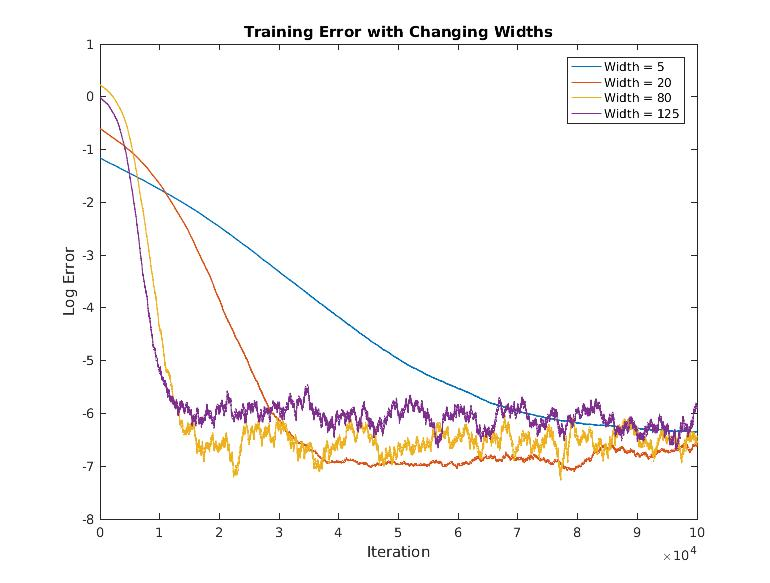
\includegraphics[width = 4.5in]{plotChangeWidth.jpg}
\caption{Test Error of Depth 2 Networks of Varying Width.}
\label{expconverge}
%  \fbox{\rule[-.5cm]{0cm}{4cm} \rule[-.5cm]{4cm}{0cm}}
\end{figure}

% Our experimental simulations show that for different widths and heights functions represented by neural networks with random edge weights can be learnt by stochastic gradient descent.
 % Our experimental simulations show that for short depths (say 2) and with random edge weights the error rate drops to a small percentage. 
%To understand this better, 



\paragraph{Results and Contributions.} 
We theoretically investigate the question of convergence for networks of depth two.
 % with certain simplifying assumptions.  
Our main conceptual contribution is that for depth $2$ networks where the top node is a sum node, the question of whether gradient descent converges to the desired target function is equivalent to the following question in electrodynamics: Given $k$ fixed protons in $\rea^d,$ and $k$ moving electrons,
% initialized at random positions 
with all the electrons moving under the influence of the 
% electrical attractive force between opposite-sign charges, and repulsive force between same-sign charges,
electrical force of attraction from the protons and repulsion from the remaining electrons,
at equilibrium, are all the electrons matched up with all the fixed protons, up to a permutation?  

In the above, $k$ is the number of hidden units, $d$ is the number of inputs, the positions of each fixed charge is the input weight vector of
% a  edge weights incident on each of the
a hidden unit in the target network, and the initial positions of the moving charges are the initial values of the weight vectors for the hidden units in the learning network. The motion of the charges essentially tracks the change in the network during gradient descent. The force between a pair of charges is not given by the standard electrical force of $1/r^2$ (where $r$ is the distance between the charges), but by a function determined by the activation and the input distribution. Thus the question of convergence in these simplified depth two networks can be resolved by studying the equivalent electrodynamics question with the corresponding force function.
%
% \Anote{If you're going to have an informal theorem statement, they should be understandable without reading the main text. That's because a reader like me will ignore your intro text and just look at the theorem statements to gauge your paper. If the theorems look interesting, then they'll read the paper. This theorem refers to f, which is undefined. it also doesn't explain at all in what way the electrons and protons correspond to f. You should either make this explicit in the informal theorem's statement, or you should just blend this informal theorem into the rest of the section.}

\begin{theorem}[informal statement of Theorem~\ref{EPDyn}]
Applying gradient descent for learning the output of a depth two network
with $k$ hidden units with activation $\sigma,$ and a linear output
node, under squared loss, using a network of the same architecture,
% two layer
% neural network 
% The gradient descent process for learning our neural network $f$ 
is equivalent to the motion of $k$ charges in the presence of $k$ fixed charges where the force between each pair of charges is given by a potential function that depends on $\sigma$ and the input distribution.  \end{theorem}
%
 % and that the training data comes from a standard multivariate Gaussian distribution.
Our main technical contribution is to prove the existence of an
activation function such that the corresponding gradient descent
dynamics under standard Gaussian inputs result in learning at least
one of the hidden nodes in the target network. We then show that this
allows us to learn the complete target network one node at a time. We
leave open the problem of convergence for dynamics corresponding to
more realistic activation functions. We assume the sample complexity
is close to its infinite limit.
%
% {\color{red} }
%We also derive the force function for several possible activation functions. }
% Further for a certain synthetic activation function, we prove that the electrodynamic force function results in convergence thus 
% implying the desired convergence for simplified depth 2 networks with those activation functions 

%
% \Anote{same problem as the other informal theorem. i don't know what a $\theta$ is. it has only been defined in the text. furthermore, it's far too informal. instead of "carefully" it should give this notion a name. again, better to just blend this content in the rest of the text without calling it an informal theorem.}
\begin{theorem}[informal statement of Theorem~\ref{almostHarmSGD}]
There is an activation function such that running gradient
  descent for minimizing the squared loss along with $\ell_2$
  regularization for standard Gaussian inputs, at convergence, 
% For some
%   carefully chosen activation function, with regularization, at
%   convergence of running the SGD algorithm, 
  we learn at least one of
  the hidden weights of the target neural network.
\end{theorem}
%
We  prove that the above result can be iterated to learn the entire network node-by-node using gradient descent (Theorem~\ref{nodeWise}).  Our algorithm learns a network with the same architecture and number of hidden nodes as the target network, 
in contrast with several existing improper learning results.
 % This is in contrast to the improper learning setting of many proposed algorithms.

In the appendix, we show some weak results for more practical activations. For the sign activation, we show that for the loss with respect to a single node, the only local minima are at the hidden target nodes with high probability if the target network has a randomly picked top layer. For the polynomial activation, we derive a similar result under the assumption that the hidden nodes are orthonormal.


 \begin{table}[h!]
 \noindent
 \vskip 0.1in
 \begin{center}
 \begin{small}
 \begin{sc}
 \begin{tabular}{
   |p{\dimexpr.28\linewidth-2\tabcolsep-1.3333\arrayrulewidth}% column 1
   |p{\dimexpr.30\linewidth-2\tabcolsep-1.3333\arrayrulewidth}% column 2
   |p{\dimexpr.42\linewidth-2\tabcolsep-1.3333\arrayrulewidth}|% column 3
   }
    \hline 
         Name of Activation&  Potential  ($\Phi(\theta,w)$)    & Convergence? \\ \hline 
        Almost   $\lambda$-harmonic  & Complicated  (see Lem~\ref{almostHarmReal}) & Yes, Thm~\ref{nodeWise}\\
         Sign & $1 - \frac{2}{\pi}\cos^{-1}(\theta^Tw)$       & Yes for d = 2, Lem~\ref{SignConv} \\   
Polynomial  & $(\theta^Tw)^m$       & Yes, for orthonormal $w_i.$ Lem~\ref{PolyStrict}  \\        
                  % Bessel    &  $e^{-\|\theta-w\|_1}$        & Yes for $d=1$  \\   
         \hline
 \end{tabular}
 \end{sc}
 \end{small}
 \end{center}
 \caption{Activation, Potentials, and Convergence Results Summary}
 \label{table1}
 \end{table} 

\paragraph{Intuition and Techniques.}
%
Note that for the standard electric potential function given by $\Phi = 1/r$ where $r$ is the distance between the charges, it is known from Earnshaw's theorem that an electrodynamic system with some fixed protons and some moving electrons is at equilibrium only when the moving electrons coincide with the fixed protons. Given our translation above between electrodynamic systems and depth 2 networks (Section~\ref{sec:epdyn}), this would imply learnability of depth 2 networks under gradient descent under $\ell_2$ loss, if the activation function corresponds to the electrostatic potential. However, there exists no activation function $\sigma$ corresponding to this $\Phi$.
%

% \paragraph{Organization.} In section 2, we introduce our framework and assumptions, and derive the equivalence between gradient descent and electron-proton dynamics under a suitable potential. 
%  % These convergence results are proven to simply illustrate our ideas. 
% In Section~\ref{}, we construct a realizable almost $\lambda$-harmonic potential and prove finite convergence guarantees. In section 6, experimental results confirm that depth-2 neural networks can be learned by gradient descent with common activation functions but seem to discredit that claim for higher depth networks. In section 5, we consider more realistic activation functions, such as the sign and polynomial function.

The proof of Earnshaw's theorem is based on the fact that the electrostatic potential is harmonic, \emph{i.e}, its Laplacian (trace of its Hessian) is identically zero. This ensures that at every critical point, there is direction of potential reduction (unless the hessian is identically zero). We generalize these ideas to potential functions that are eigenfunctions of the Laplacians, $\lambda$-harmonic potentials (Section~\ref{sec:earnshaw}). However, these potentials are unbounded. Subsequently, we construct a non-explicit activation function such that the corresponding potential is bounded and is almost $\lambda$-harmonic, \emph{i.e.}, it is $\lambda$-harmonic outside a small sphere (Section~\ref{sec:almost-harmonic}). For this activation function, we show at a stable critical point, we must learn at least one of the hidden nodes. Gradient descent (possibly with some noise, as in the work of Ge \emph{et al.}~\cite{GeHJY15}) is believed to converge to stable critical points. However, for simplicity, we descend along directions of negative curvature to escape saddle points. Our activation lacks some regularity conditions required in~\cite{GeHJY15}. We believe the results in \cite{jin2017escape} can be adapted to our setting to prove that perturbed gradient descent converges to stable critical points.

% $M_{G,\epsilon}$ but requires more in-depth analysis.

%\Snote{We use recent results on gradient descent~\cite{Rongetal} to show that gradient descent (with perturbations) converges close a stable critical point.}

% {\color{red}The use of second-order methods is not limiting since noisy gradient descent algorithms can descent along negative curvature directions. Therefore, stochastic gradient descent should also converge to $M_{G,\epsilon}$, although we lack some regularity conditions. Furthermore, a more controlled perturbed gradient descent }


% Our main tool for analysis is to derive second-order information about our dynamics by using the Laplacian of the Hessian (or a submatrix of the Hessian) of our loss function. 
% Together with some generalization error bounds and discrete optimization results, we can finally translate these convergence results into finite time convergence rates. 


% We derive some sufficient conditions that characterize potentials
%  that arise from activation functions $\sigma$. 

% The different $\sigma$ that we study, their corresponding potentials, and their convergence results are summarized in Table ~\ref{table1}.
% First we show how to construct an activation function, such that the corresponding potential satisfies a nice smooth property which we call almost $\lambda$-harmonic, 
% for which we show that at convergence of the gradient descent, at least some $\theta_i$ coincides with some $w_j$.
%

%
%


There is still a large gap between theory and practice. However, we believe our work can offer some theoretical explanations and guidelines for the design of better activation functions for gradient-based training algorithms. For example, better accuracy and training speed were reported when using the newly discovered exponential linear unit (ELU) activation function in \cite{ClevertUH15, ShahKSS16}. We hope for more theory-backed answers to these and many other questions in deep learning.



%%% Local Variables:
%%% mode: latex
%%% TeX-master: "icmlpaper2017.tex"
%%% End:
